\chapter{Basics}

\section{Definitions}

In this script we will use the terms '1', TRUE and HIGH synonymously. Similarly, we will use '0', FALSE and LOW. Further 
we will use two's complement for signed binary numbers.

\section{Design and Choices}

Microprocessors where and still are a fundamental building block for the technological progess in the past
three decades. Without them things like the Internet and cell phones would not exist. But for the
development of new chips performance is not always the main priority. While performance is important,
there is always a tradeoff between many different other aspects, including power consumption, temperature
price and size, only to mention some of them.

Systems like a microprocessor can get really complicated to understand on a low level. To get a better
understanding of such a system, it is necessary to use different techniques:
\begin{itemize}
    \item Abstraction: hiding details when they are not important
    \item Disciplin: intentionally restricting design choices so that you can work more productively at a higher level of abstraction
    \item Hierarchy, Modularity, Regularity: defining a clear structure dividing a system into well-defined modules and reusing them among multiple points
\end{itemize} 

Microarchitecture links the logic and architecture levels of abstraction. This will be the main focuse of this course.

\begin{figure}[h]
    \centering
    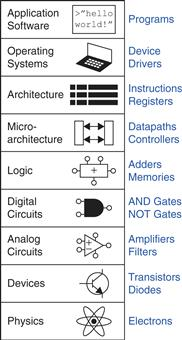
\includegraphics[width=3cm]{abstractionLevels.jpg}
    \caption{Levels of abstraction for a electronic computing system}
\end{figure}

\pagebreak

\section{Representing Numbers}

There are three commonly used systems to represent numbers. We normally use decimal numbers, but
in digital systems binary and hexadecimal numbers are more convienient. It is assumed that the reader
is familiary with using these number systems and knows how to performe simple operations in them. When
dealing with addition one has to be carefull to check for overflow of the carry bit.

\begin{satz}[Important Terms]
    \begin{itemize}
        \item \textbf{Bit}: A single 0 or 1
        \item \textbf{Byte}: A group of eight bits, can be represented by two hexadecimal digit
        \item \textbf{Nibble}: Half a byte, can be represented by one hexadecimal digit
        \item \textbf{Word}: Data chunks a microprocessor handels, today 64 or 32 bit
        \item \textbf{LSB}: least significant bit, right-most bit in a group of bits
        \item \textbf{MSB}: most significant bit, left-most bit in a group of bits
    \end{itemize}
\end{satz}

There are multiple ways to represent a negative number in the binary system. The two most common ones are
called sign/magnitude and two's complement.

\textbf{Sign/Magnitude}: We use the MSB as a sign bit, this causes the problems that addition will no longer work
and there exists both $+0$ and $-0$. This covers the range $[-2^{N-1}+1, 2^{N-1}-1]$.

\textbf{Two's Complement}: Same system as a unsigned binary number except the MSB has a weight of $-2^{N-1}$.
Here addition works fine and there is only one representation for $0$. The process of creating a negative number
consists of inverting all the bits of the number and adding $1$ to the LSB. This covers the range $[-2^{N-1}, 2^{N-1}-1]$.

\section{Logic Gates}

Logic Gates are simple digital circuits that take one or more binary inputs (denoted by letters from the beginning of the alphabet) and 
produce a binary output (commonly denoted Y). The most common logic gates are:

\begin{figure}[h]
    \centering
    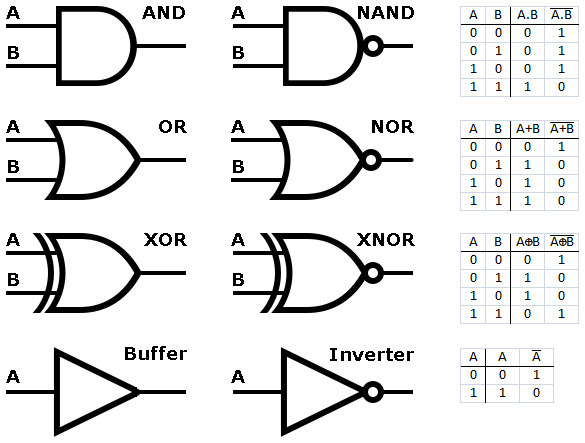
\includegraphics[width=9cm]{gates.png}
    \caption{Most important logic gates}
\end{figure}

Note that a N-input XOR produces a TRUE output when an odd number of inputs are TRUE. From a logical point of view, a buffer 
might seem useless. However, from the analog point of view, the buffer has multiple, desirable characteristics such as the 
ability to quickly send its output to many gates. The logic operations can be denoted as follows:

\begin{center}
    \begin{tabular}{ c  l }
        BUFFER & $Y = A$  \\ 
        NOT & $Y = \overline{A}$  \\ 
        AND & $Y = A \cdot B = AB = A \cap  B$  \\ 
        OR & $Y = A + B = A \cup B $  \\ 
        XOR & $Y = A \oplus B$  \\ 
        NAND & $Y = \overline{AB}$  \\   
        NOR & $Y = \overline{A + B}$ \\
        XNOR & $Y = \overline{A \oplus B}$
    \end{tabular}
\end{center}

There also exist logic gates with more than two inputs.

\section{Beneath the Abstraction}

\paragraph{Supply Voltage:} In reality, binary signals are represented with a voltage on a wire. The lowest
voltage in a system (0 V) is called the ground GND and the highest is denotes as $V_{DD}$ (between 1.2 and 3.3 V).

\paragraph{Noise:} Since in reality this signal is analog and could theoretically have every value between GND and $V_{DD}$ it could
be that we encounter noise. We can use a trick to filter such noise and get a clear signal. The noise margin
is the amount of noise we can add to a signal and it can still be correctly interpreted. In this example we look
at two simple logic gates, a driver and receiver. The noise margin is calculated $NM_L = V_{IL} - V_{OL}$, 
$NM_H = V_{OH} - V_{IH}$.

\begin{figure}[h]
    \centering
    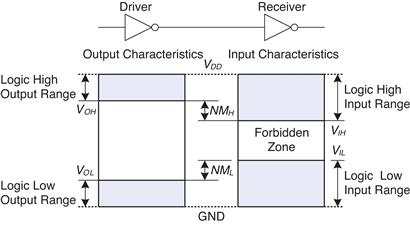
\includegraphics[width=11cm]{noise.jpg}
    \caption{Noise characteristics}
\end{figure}

\paragraph{CMOS Transistors:} We skip the detailed explanation of how a transistor works and look at what it does.
A transistor can be viewed as a electrically controlled switch that turns ON or OFF when a voltage is applied to a
controll terminal. The most common transistors are MOS transistors (or MOSFET). There are two types nMOS and pMOS.
\pagebreak
\begin{figure}[h]
    \centering
    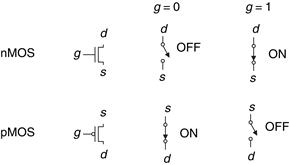
\includegraphics[width=11cm]{mosfet.jpg}
    \caption{MOS transistors}
\end{figure}
\pagebreak

\paragraph{Logic Gates:} We can use transistor to build logic gates, as an example we will have a look at how a AND gate is
built. A AND gate consists of a NAND gate and a NOT gate, that are made up by transistors as can be seen in the figure.

\begin{figure}[h]
    \centering
    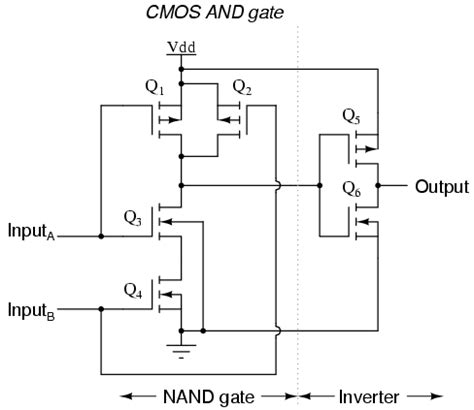
\includegraphics[width=10cm]{cmosAnd.jpeg}
    \caption{MOS transistors}
\end{figure}